\documentclass[14pt]{extbook}
\usepackage{multicol, enumerate, enumitem, hyperref, color, soul, setspace, parskip, fancyhdr} %General Packages
\usepackage{amssymb, amsthm, amsmath, latexsym, units, mathtools} %Math Packages
\everymath{\displaystyle} %All math in Display Style
% Packages with additional options
\usepackage[headsep=0.5cm,headheight=12pt, left=1 in,right= 1 in,top= 1 in,bottom= 1 in]{geometry}
\usepackage[usenames,dvipsnames]{xcolor}
\usepackage{dashrule}  % Package to use the command below to create lines between items
\newcommand{\litem}[1]{\item#1\hspace*{-1cm}\rule{\textwidth}{0.4pt}}
\pagestyle{fancy}
\lhead{Progress Quiz 6}
\chead{}
\rhead{Version C}
\lfoot{4563-7456}
\cfoot{}
\rfoot{Summer C 2021}
\begin{document}

\begin{enumerate}
\litem{
Determine the vertical asymptotes and holes in the rational function below.\[ f(x) = \frac{9x^{3} -36 x^{2} +17 x + 30}{12x^{2} -11 x -15} \]\begin{enumerate}[label=\Alph*.]
\item \( \text{Vertical Asymptotes of } x = -0.75 \text{ and } x = 1.667 \text{ with no holes.} \)
\item \( \text{Vertical Asymptotes of } x = -0.75 \text{ and } x = -0.667 \text{ with a hole at } x = 1.667 \)
\item \( \text{Holes at } x = -0.75 \text{ and } x = 1.667 \text{ with no vertical asymptotes.} \)
\item \( \text{Vertical Asymptote of } x = -0.75 \text{ and hole at } x = 1.667 \)
\item \( \text{Vertical Asymptote of } x = 0.75 \text{ and hole at } x = 1.667 \)

\end{enumerate} }
\litem{
Determine the vertical asymptotes and holes in the rational function below.\[ f(x) = \frac{12x^{3} +41 x^{2} -38 x -40}{9x^{2} +18 x + 8} \]\begin{enumerate}[label=\Alph*.]
\item \( \text{Vertical Asymptotes of } x = -1.333 \text{ and } x = -0.667 \text{ with no holes.} \)
\item \( \text{Vertical Asymptote of } x = -1.333 \text{ and hole at } x = -0.667 \)
\item \( \text{Holes at } x = -1.333 \text{ and } x = -0.667 \text{ with no vertical asymptotes.} \)
\item \( \text{Vertical Asymptote of } x = 1.333 \text{ and hole at } x = -0.667 \)
\item \( \text{Vertical Asymptotes of } x = -1.333 \text{ and } x = 1.25 \text{ with a hole at } x = -0.667 \)

\end{enumerate} }
\litem{
Which of the following functions \textit{could} be the graph below?
\begin{center}
    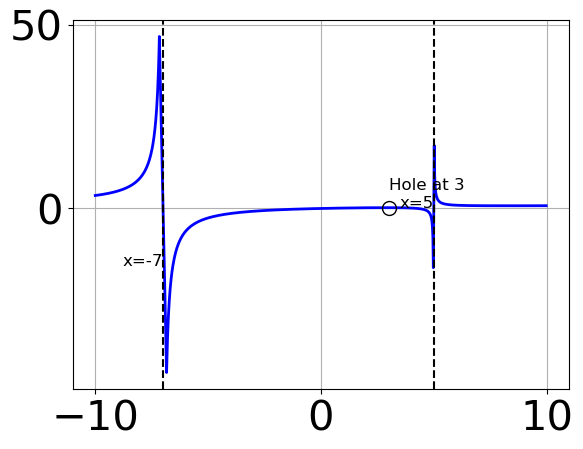
\includegraphics[width=0.5\textwidth]{../Figures/identifyGraphOfRationalFunctionCopyC.png}
\end{center}
\begin{enumerate}[label=\Alph*.]
\item \( f(x)=\frac{x^{3} -21.0 x + 20.0}{x^{3} -1.0 x^{2} -41.0 x + 105.0} \)
\item \( f(x)=\frac{x^{3} +12.0 x^{2} +39.0 x + 28.0}{x^{3} + x^{2} -41.0 x -105.0} \)
\item \( f(x)=\frac{x^{3} -8.0 x^{2} +19.0 x -12.0}{x^{3} -1.0 x^{2} -41.0 x + 105.0} \)
\item \( f(x)=\frac{x^{3} +8.0 x^{2} +19.0 x + 12.0}{x^{3} + x^{2} -41.0 x -105.0} \)
\item \( \text{None of the above are possible equations for the graph.} \)

\end{enumerate} }
\litem{
Determine the horizontal and/or oblique asymptotes in the rational function below.\[ f(x) = \frac{4x^{3} -16 x^{2} -9 x + 36}{2x^{2} -3 x -9} \]\begin{enumerate}[label=\Alph*.]
\item \( \text{Horizontal Asymptote of } y = 2.0  \)
\item \( \text{Horizontal Asymptote at } y = 3.0 \)
\item \( \text{Horizontal Asymptote of } y = 2.0 \text{ and Oblique Asymptote of } y = 2x -5 \)
\item \( \text{Oblique Asymptote of } y = 2x -5. \)
\item \( \text{Horizontal Asymptote of } y = 3.0 \text{ and Oblique Asymptote of } y = 2x -5 \)

\end{enumerate} }
\litem{
Determine the horizontal and/or oblique asymptotes in the rational function below.\[ f(x) = \frac{4x^{3} -19 x + 15}{2x^{2} +x -10} \]\begin{enumerate}[label=\Alph*.]
\item \( \text{Horizontal Asymptote of } y = 2.0  \)
\item \( \text{Horizontal Asymptote of } y = 2.0 \text{ and Oblique Asymptote of } y = 2x -1 \)
\item \( \text{Horizontal Asymptote of } y = 2.0 \text{ and Oblique Asymptote of } y = 2x -1 \)
\item \( \text{Oblique Asymptote of } y = 2x -1. \)
\item \( \text{Horizontal Asymptote at } y = 2.0 \)

\end{enumerate} }
\litem{
Determine the horizontal and/or oblique asymptotes in the rational function below.\[ f(x) = \frac{5x^{2} +22 x + 8}{25x^{3} -50 x^{2} -4 x + 8} \]\begin{enumerate}[label=\Alph*.]
\item \( \text{Oblique Asymptote of } y = 5x -32. \)
\item \( \text{Horizontal Asymptote of } y = 0.200  \)
\item \( \text{Horizontal Asymptote of } y = 0.200 \text{ and Oblique Asymptote of } y = 5x -32 \)
\item \( \text{Horizontal Asymptote at } y = -4.000 \)
\item \( \text{Horizontal Asymptote of } y = 0 \)

\end{enumerate} }
\litem{
Determine the vertical asymptotes and holes in the rational function below.\[ f(x) = \frac{6x^{3} -1 x^{2} -47 x + 30}{6x^{2} +5 x -6} \]\begin{enumerate}[label=\Alph*.]
\item \( \text{Vertical Asymptotes of } x = -1.5 \text{ and } x = 2.5 \text{ with a hole at } x = 0.667 \)
\item \( \text{Vertical Asymptote of } x = 1.0 \text{ and hole at } x = 0.667 \)
\item \( \text{Vertical Asymptotes of } x = -1.5 \text{ and } x = 0.667 \text{ with no holes.} \)
\item \( \text{Vertical Asymptote of } x = -1.5 \text{ and hole at } x = 0.667 \)
\item \( \text{Holes at } x = -1.5 \text{ and } x = 0.667 \text{ with no vertical asymptotes.} \)

\end{enumerate} }
\litem{
Determine the horizontal and/or oblique asymptotes in the rational function below.\[ f(x) = \frac{5x^{2} -27 x + 10}{15x^{3} -31 x^{2} -50 x + 24} \]\begin{enumerate}[label=\Alph*.]
\item \( \text{Oblique Asymptote of } y = 3x + 10. \)
\item \( \text{Horizontal Asymptote of } y = 0.333 \text{ and Oblique Asymptote of } y = 3x + 10 \)
\item \( \text{Horizontal Asymptote of } y = 0.333  \)
\item \( \text{Horizontal Asymptote of } y = 0 \)
\item \( \text{Horizontal Asymptote at } y = 5.000 \)

\end{enumerate} }
\litem{
Which of the following functions \textit{could} be the graph below?
\begin{center}
    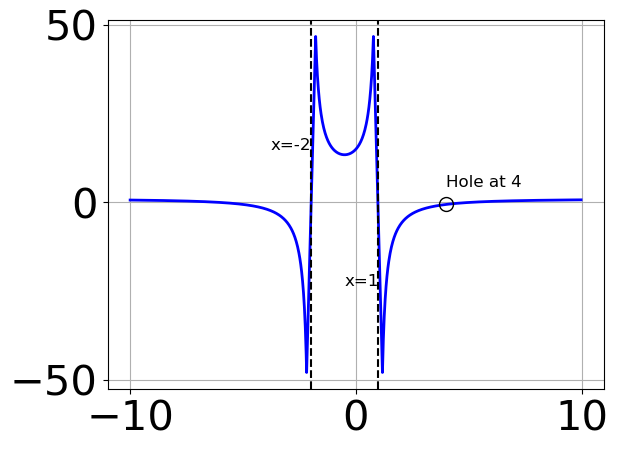
\includegraphics[width=0.5\textwidth]{../Figures/identifyGraphOfRationalFunctionC.png}
\end{center}
\begin{enumerate}[label=\Alph*.]
\item \( f(x)=\frac{x^{3} -3.0 x^{2} -34.0 x + 120.0}{x^{3} -3.0 x^{2} -6.0 x + 8.0} \)
\item \( f(x)=\frac{x^{3} +3.0 x^{2} -34.0 x -120.0}{x^{3} +3.0 x^{2} -6.0 x -8.0} \)
\item \( f(x)=\frac{x^{3} +2.0 x^{2} -33.0 x -90.0}{x^{3} +3.0 x^{2} -6.0 x -8.0} \)
\item \( f(x)=\frac{x^{3} -5.0 x^{2} -36.0 x + 180.0}{x^{3} -3.0 x^{2} -6.0 x + 8.0} \)
\item \( \text{None of the above are possible equations for the graph.} \)

\end{enumerate} }
\litem{
Determine the vertical asymptotes and holes in the rational function below.\[ f(x) = \frac{6x^{3} -23 x^{2} +9 x + 18}{6x^{2} +19 x + 10} \]\begin{enumerate}[label=\Alph*.]
\item \( \text{Vertical Asymptotes of } x = -2.5 \text{ and } x = 1.5 \text{ with a hole at } x = -0.667 \)
\item \( \text{Holes at } x = -2.5 \text{ and } x = -0.667 \text{ with no vertical asymptotes.} \)
\item \( \text{Vertical Asymptotes of } x = -2.5 \text{ and } x = -0.667 \text{ with no holes.} \)
\item \( \text{Vertical Asymptote of } x = 1.0 \text{ and hole at } x = -0.667 \)
\item \( \text{Vertical Asymptote of } x = -2.5 \text{ and hole at } x = -0.667 \)

\end{enumerate} }
\end{enumerate}

\end{document}